\section{The FSM Driver}\label{sec:fsm}
The proposal for controlling the car is a \emph{Finite State Machine}, which
enables a modular development, ideal for teamwork, and separates behaviors, reducing
the effort necessary to evolve a complete controller by breaking this problem into
evolving each state.

From the intuitive perspective of a human driver in a car race competition, there 
is a clearly defined desirable behavior: to \emph{drive faster than the competitors}.
The simulation account for different environment conditions, therefore a car's 
performance is always better, everything else being the same, when it is within 
track limits than outside. So this rather complex behavior which can be broken into specific behaviors: \emph{drive as fast as possible on the track} and, 
in case something goes wrong, \emph{get back on the track as fast as possible}.

Driving as fast as possible on a straight line is simple, but a different behavior
than doing it in a curve, thus the state can be further divided into \emph{drive
drive as fast as possible in a straight line} and \emph{make the
curve as fast as possible}. Finally, because racing usually implies being able to
move forward, a behavior for handling situations when that is not possible is 
necessary.

\begin{figure}
	\centering
	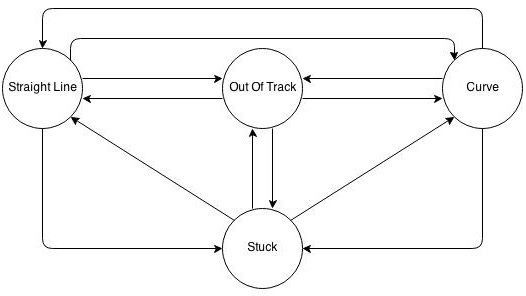
\includegraphics[width=3in]{StatesDiagram}
	\caption{State transition diagram.}
	\label{fig:fsm}
\end{figure}

Therefore, FSMDriver's initial configuration has four states, as illustrated in 
Fig. \ref{fig:fsm}, described as follows: 

\begin{itemize}
	\item \textbf{Straight Line}: the controller commands the car to full throttle 
	with maximum acceleration straight ahead, adjusting the steering to stay in 
	the middle of the track.
	
	\item \textbf{Curve}: the controller handles curves based on the position of 
	the car and the angle between the direction of the axes of the car and the 
	track axis, adjusting the steering, gear, and clutch actuators to keep it 
	moving as fast as possible within track limits while trying to avoid damage
	(by crashing into another car or wall).
	
	\item \textbf{Out of Track}: the controller tries to return to the 
	track as fast as possible by steering in an arbitrary angle (with 
	relation to the track's axis of track). Due to low friction outside of the 
	track, accelerating and braking are proportional to the sideway speed of the 
	car to minimize skidding.
	
	\item \textbf{Stuck}: the controller takes drastic measures to try to recover, 
	using reverse gear and hard steering to try to get back on track in this worst 
	case scenario.
\end{itemize}

There are two states for usual on track regular on track situations and two for
off track ones. Only one of these states will be in control at a time, but all 
have to work together to handle the all possible scenarios and each has to be
properly configured to achieve competitive results.

The complete behavior is achieved by transitioning between states, this is 
implemented in a \texttt{transition} function that uses specific parameters to decide when 
the current state needs to be changed (and which state to change to). This function 
operates on four constant parameters:
	\begin{itemize}
		\item[$MSD$,] the maximum speed distance, which defines the 
		maximum value for the frontal sensor input while racing at full speed;
		\item[$LE$,] the track's left edge boundary, which defines the area
		available for moving the car left;
		\item[$RE$,] the track's right edge boundary, which defines the area
		available for moving the car right;
		\item[$ST$,] the number of stuck ticks, required by the controller 
		for identifying how long it has not been moving fast enough and, thus,
		concluding it is stuck.
	\end{itemize}

\texttt{transition} analyses the car's inputs to define if there has to be a
change in state on every simulation tick. The first procedure is to check if the
car is \textbf{Stuck}, that is, if it is has a very low speed (obviously, ignoring 
the beginning of the race when all cars ares stopped), then a counter is incremented 
and its value compared to the $ST$ threshold.

In case the car is not stuck, \texttt{transition} will define the current state
by analyzing its position in the track. It will be \textbf{Out of Track} if it is
out of the range defined by $LE$ and $RE$. Otherwise, it is considered 
on track and can be either on a \textbf{Straight Line}, if the frontal distance 
sensor's input is larger than $MSD$ or when it is larger than the input of the 
adjacent side sensors, or on a \textbf{Curve} otherwise. 